\chapter{Preliminaries}
\label{chap:prelim}

\begin{figure}
	\centering
	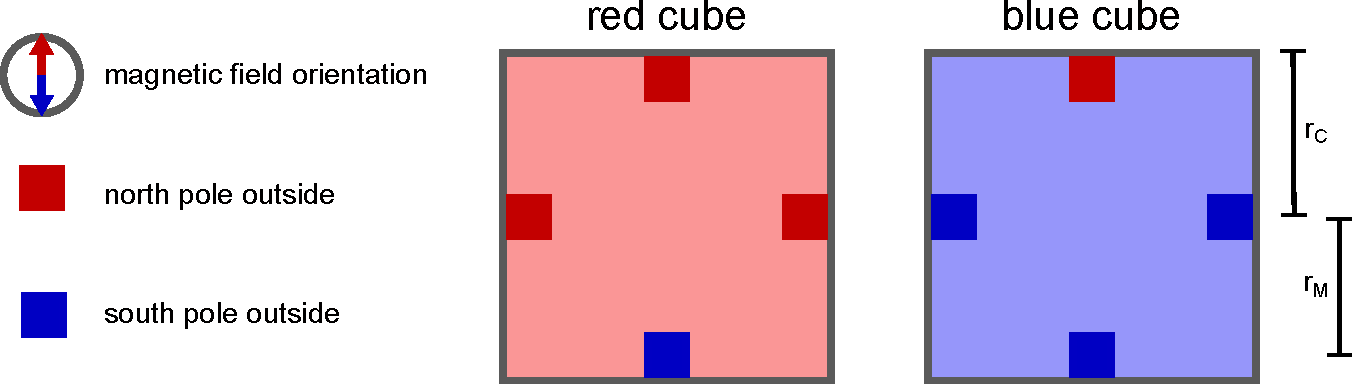
\includegraphics[width=0.75\textwidth]{figures/magnetic_cubes.pdf}
	\caption[Top-down view of the two magnetic modular cube types]{Simplified top-down view of the two magnetic modular cube types with their outward pointing magnet poles, illustrated as red and blue squares. Also visualizes the lengths $r_C$ and $r_M$}
	\label{fig:magnetic_cubes}
\end{figure}

\section{Magnetic Modular Cubes}
The magnetic modular cubes are cube-shaped bodies embedded with permanent magnets on the four side faces.
The magnets have different orientations of their north and south pole. 
One pole is always pointing outside and the other straight to the center of the cube.
The magnet at the front face has its north pole pointing outwards and the magnet at the back its south pole.
These two magnets ensure that the cube is always aligned with the global magnetic field and this orientation holds true for both cube types.
The two other side faces must have the same outwards pointing pole, so that it is not possible for this axis to align with the magnetic field.

In fact, this is the reason a distinct definition of front, back and side is even possible.
Since the front is always pointing to the north pole of the magnetic field, we also call it the north face, or north edge in two dimensions, and all the other faces can also be called by their corresponding cardinal direction.
For each face we define a vector $\vec{e} \in \{ \vec{N},\vec{E},\vec{S},\vec{W}\}$ with $\lVert \vec{e} \rVert = 1$ pointing in the cardinal direction of the magnetic field.
For simplification we call magnets by their outwards pointing pole in further sections.

Furthermore, two different cube types are defined:
Either both side magnets point out their north pole, these cubes are called red cubes, or they point out their south pole, which is then called a blue cube.
\autoref{fig:magnetic_cubes} shows a top-down view of the two cube types with all the outwards pointing magnet poles.
A compass always shows the orientation of the magnetic field in our illustrations.

Magnetic Modular Cubes can be constructed in different sizes and ways. For more technical details and length measurements, we refer to the original \cite{Bhattacharjee2022}.
Two important lengths that we use for planning and simulating are the cube radius $r_C$ and the magnet radius $r_M$ (also illustrated in \autoref{fig:magnetic_cubes}).
$r_C$ is one half-length of a cube face and $r_M$ is the distance from the center of the cube to the center of the magnet.

\begin{figure}
	\centering
	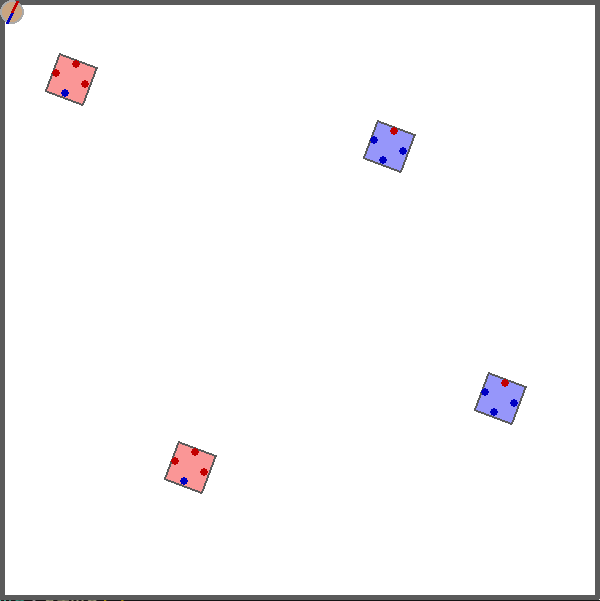
\includegraphics[width=0.53\textwidth]{figures/workspace_config.png}
	\caption[Workspace with a configuration of four magnetic modular cubes]{Rectangular workspace with a configuration of four magnetic modular cubes. All cubes have the same orientation as the magnetic field, indicated by the compass in the top-left corner.}
	\label{fig:workspace_config}
\end{figure}

\section{Workspace and Configuration}
Magnetic modular cubes could theoretical be placed and maneuvered on any 2-dimensional plane with numerous obstacles, as long as you can surround the workspace with a time varying magnetic field.
The magnetic field should be able to point in any direction specified by angles of latitude and longitude, so that the cubes can operate in all desired motion modes.
Because the motion planning problem of self-assembling target shapes in the special Euclidean group is hard enough without considering obstacles and arbitrary workspace shapes, we only work in a rectangular workspace with no internal obstacles.
The workspace is limited by surrounding walls, which are the only objects that could be considered as obstacles in classical motion planning.
However, we do not assume a fixed size, as long as the workspace stays finite and rectangular.

For planning we work in the configuration space of the 2-dimensional special Euclidean group $SE(2) = \mathbb{R}^2 \times \mathbb{S}^1$.
When only considering one cube, the group consists of the position in $\mathbb{R}^2$ and an orientation $\mathbb{S} = [0,2\pi)$ \cite{LaValle2006}.
When working with $n$ cubes, the dimension of our configuration space increases to $\mathbb{R}^{2n} \times \mathbb{S}^1$.
Note that we can still assume only one orientation for $n$ cubes, because we are working with a global magnetic field orienting all cubes the same way.
\autoref{fig:workspace_config} shows a configuration with four cubes in the workspace.
It is irrelevant which exact physical cube is at which position as long as they are the same type, so switching the positions of the two red cubes in \autoref{fig:workspace_config} would lead to the same configuration as before.

\begin{figure}
	\centering
	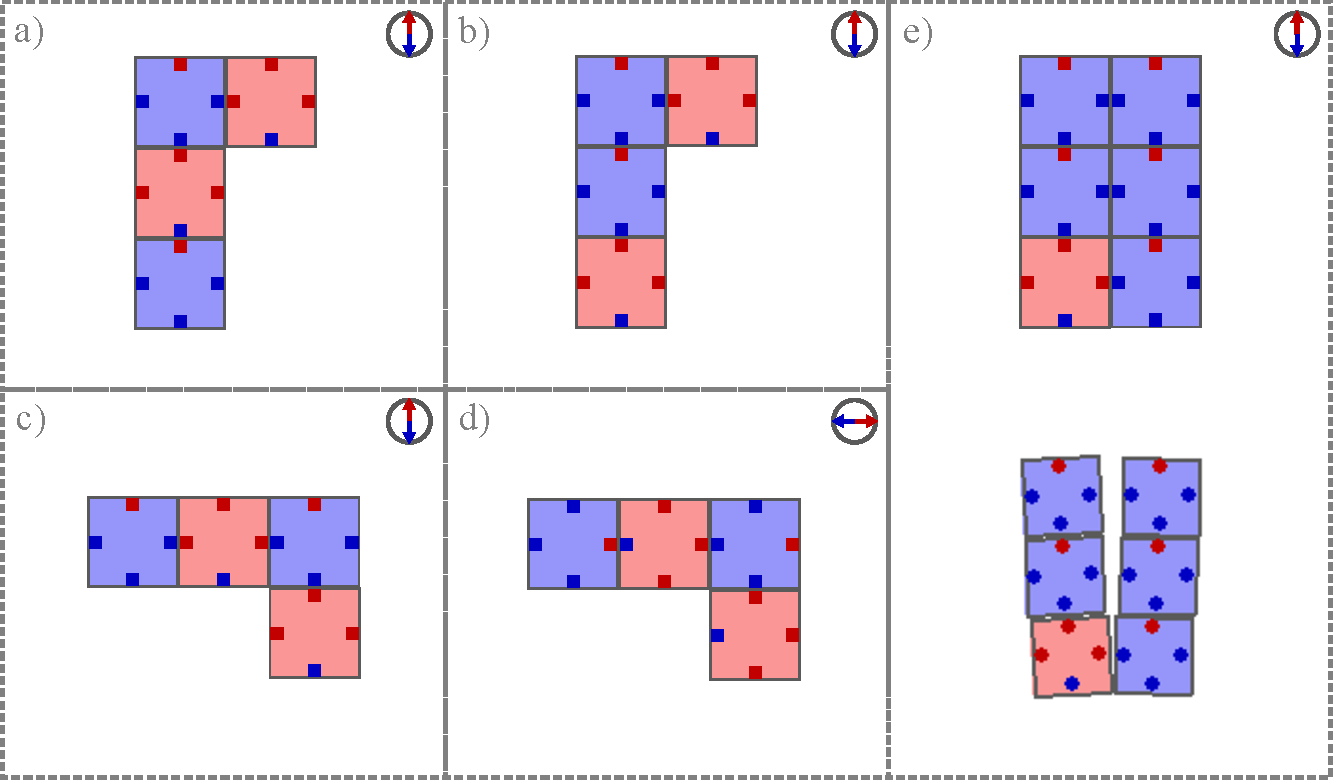
\includegraphics[width=0.65\textwidth]{figures/polyominoes.pdf}
	\caption[Examples of Polyominoes and their equality]{Examples of polyominoes and their equality. a) and d) are equal, only the magnetic field changed its orientation. a) and c) are not equal, they have the same shape but rotated. a) and c) are also not equal because of different cube types in the same shape. e) shows an invalid polyomino in its grid representation (top) and how it behaves in the simulation (bottom).}
	\label{fig:polyominoes}
\end{figure}

\section{Polyominoes}
\label{sec:polys}
The embedded magnets not only align the cube with the magnetic field, they also allow cubes to self-assemble into polyominoes.
Two cube faces can connect if their magnets have opposite polarities.
Because of this and the alignment with the magnetic field, cubes can either be connected at north and south faces, or east and west faces, if the cubes are not the same type.
A polyomino is a set of uniformly sized cubes on a 2-dimensional grid.
Because we work with arbitrary positions and orientations the grid alignment does not hold true for multiple polyominoes in the workspace, but for each polyomino on its own the cubes can be represented in a local coordinate system with position $(x,y)$, $x,y \in \mathbb{Z}$ \cite{Lu2021}.

We consider fixed polyominoes, meaning that two polyominoes are distinct if their shape or orientation are different \cite{Lu2021}.
The magnetic field always provides an orientation, so in \autoref{fig:polyominoes} a) and d) the polyominoes are equal, just the magnetic field is rotated.
Conversely, the polyominoes in \autoref{fig:polyominoes} a) and c) are the same shape but with a different rotation under the same magnetic field orientation, so they are not equal.
Furthermore, two polyominoes are only equal if all the cubes at equal positions are the same type.
The polyominoes in \autoref{fig:polyominoes} a) and b) are not equal because the cube types differ.
It is possible that a workspace contains multiple equal polyominoes.
In that case, we refer to them as being the same polyomino-type, instead of calling them equal, since it is important to differentiate between physical polyominoes with different positions.

The size of a polyomino is the number of cubes it consists of.
Because it is easier to view all structures in the workspace as a polyomino, single cubes are often referred to as trivial polyominoes with size 1.
Although it is not possible to connect cubes of same type at east and west faces, the magnetic modular cubes can assemble structures like the one shown in \autoref{fig:polyominoes} e).
The connection of the bottom two cubes is strong enough to hold the structure together, even though the four blue cubes on the top repel each other.
The resulting polyomino in its grid representation has two east-west connections between cubes the same type and is therefor marked as an invalid polyomino.

\begin{figure}
	\centering
	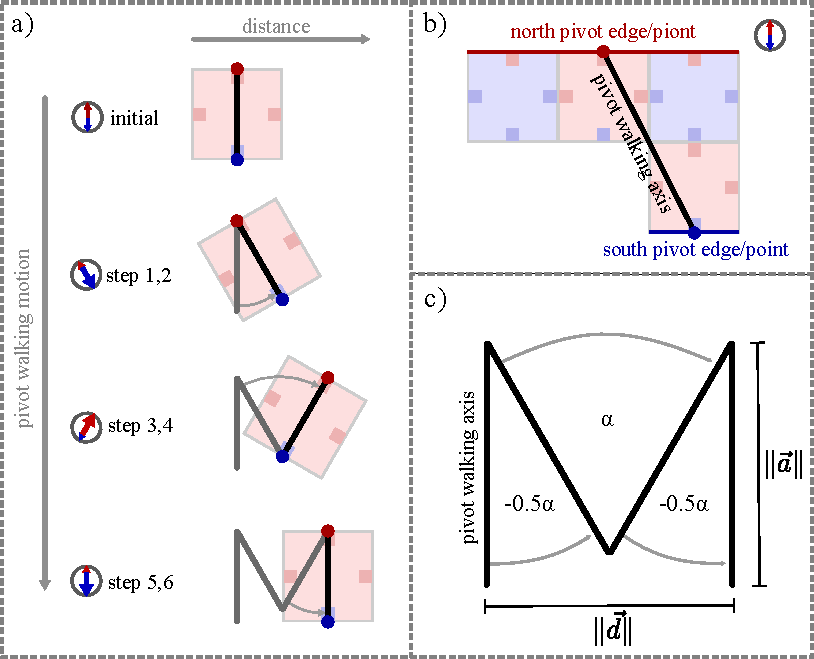
\includegraphics[width=0.80\textwidth]{figures/pivot_walking.pdf}
	\caption[Illustration of the pivot walking motion]{This figure describes the pivot walking motion in detail. a) shows the six pivot walking steps for a single red cube. You can see the orientation of the magnetic field (bigger arrow indicates elevation). In b) an example polyomino with its pivot axis, edges and points is shown. c) illustrates the rotation of the pivot axis labeled with all the pivot walking parameters.}
	\label{fig:pivot_walking}
\end{figure}

\section{Motion Modes}
\label{sec:motion}
In \cite{Bhattacharjee2022} three motion modes are presented. Rotation, pivot walking and rolling.

If the magnetic field orientation lays in the plane of the workspace and rotates without any inclination the rotation is performed around the center of mass for all polyominoes and we consider this motion a normal rotation.

Rotating the magnetic field perpendicular to the workspace plane, cubes can roll forwards or backwards.
This rolling motion becomes problematic for self-assembly, because the top and bottom face of the cube, which contain no magnets, can become a side face.
Because rotation and pivot walking are sufficient to reach any position in the workspace, we do not consider rolling in our simulation and planning algorithms.

When elevating the magnetic field orientation by lifting up the south pole slightly, all polyominoes will pivot on the north face bottom edges of their most north-placed cubes.
Pulling up the north pole does the opposite. The polyominoes will pivot on the south face bottom edges of their most south-placed cubes.
The sum of all these cube edges is called the north or south pivot-edge and by keeping the magnetic field elevated and rotating around the normal vector of the workspace plane, the polyominoes will rotate around the center point of their pivot-edge.
This point is called the north or south pivot-point.
All these edges and points are illustrated in \autoref{fig:pivot_walking} b).

\begin{figure}
	\centering
	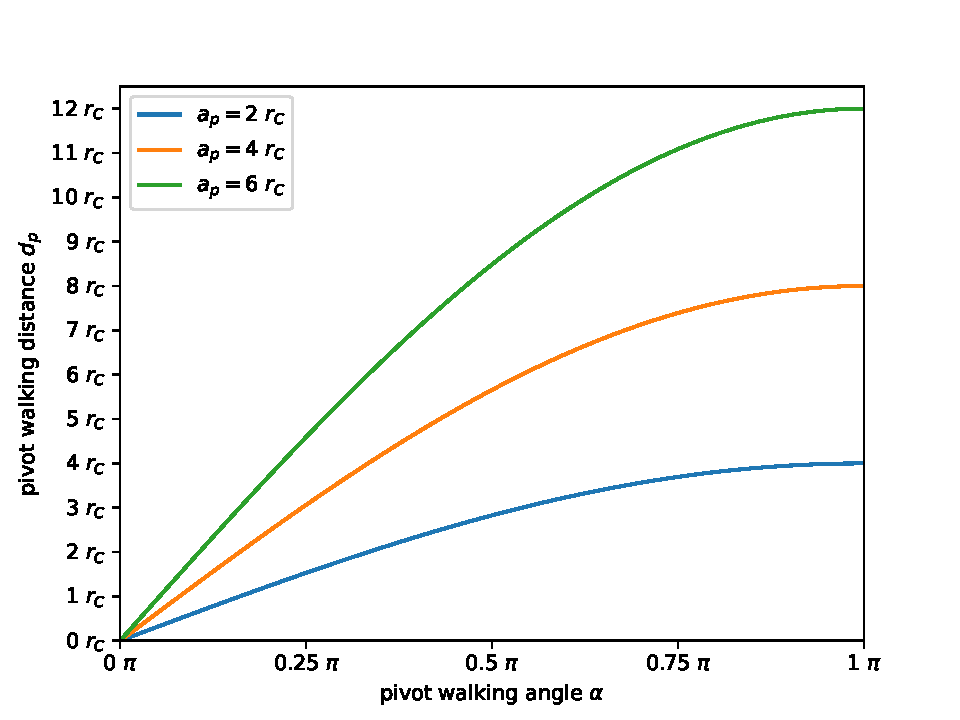
\includegraphics[width=0.70\textwidth]{figures/plots/pivot_walking_angle.pdf}
	\caption[Functions of $d_p$ based on $\alpha$ for different $a_p$]{Functions of the pivot walking distance $d_p$ based on pivot walking angle $\alpha$ for different pivot walking axes with length $a_p$. Length are giveen in multiples of cube radius $r_C$.}
	\label{fig:pw_angle_plot}
\end{figure}

\begin{figure}
	\centering
	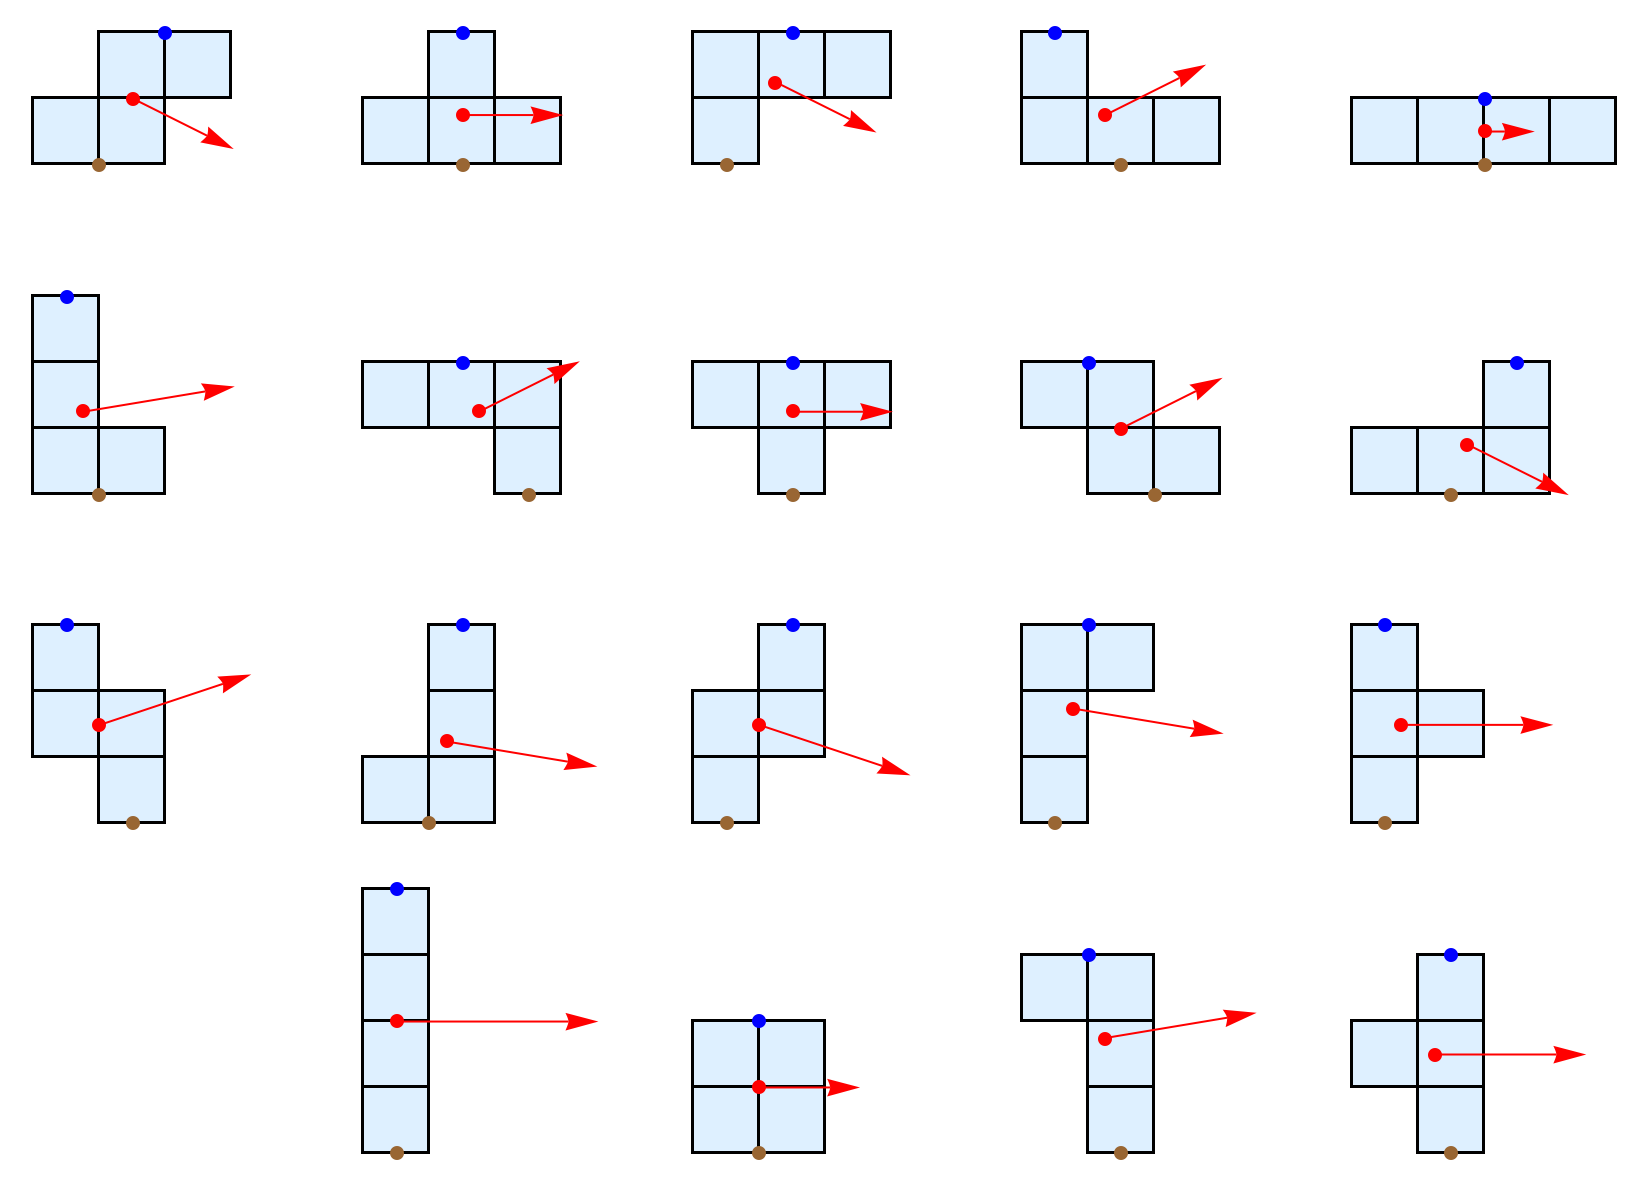
\includegraphics[width=0.70\textwidth]{figures/displacement_pivot_walking.png}
	\caption[Polyomino shapes with different displacement vectors]{All 19 four-cube polyomino shapes with their displacement vector $\vec{d}$ for one pivot walking cycle with $\alpha = \frac{\pi}{4}$. $\vec{d}$ is drawn from the center of mass (red dot). North and south pivot point are drawn as blue and brown dots.}
	\label{fig:displacement_pivot_walking}
\end{figure}

\paragraph{pivot walking:}
Not rotating around the center of mass is important for pivot walking.
In the first step of a pivot waking cycle, the magnetic field is elevated to let the polyomino pivot on its north pivot edge.
As a second step a rotation of $-\frac{1}{2} \cdot \alpha$ is performed around the north pivot point.
$-\pi \leq \alpha \leq \pi$ is the pivot walking angle.
For step 3 and 4 the elevation changes to its opposite to perform a rotation of $\alpha$ around the south pivot point.
Step 5 and 6 are equal to 1 and 2 and will bring the polyomino back to its original orientation.
You can see the pivot walking cycle steps in \autoref{fig:pivot_walking} a) and have a closer look at its parameters in \autoref{fig:pivot_walking} c).

After one pivot walking cycle, the polyomino has moved by a displacement vector $\vec{d}$ with $\lVert \vec{d} \rVert = d_p$, so $d_p$ is the distance the polyomino moved.
The direction and length of $\vec{d}$ changes with the shape of the polyomino.
The movement is always perpendicular to the pivot walking axis $\vec{a}$ with $\lVert \vec{a} \rVert = a_p$, which is the vector between the north and the south pivot point, visualized in \autoref{fig:pivot_walking} b).
$d_p$ can be calculated as
\begin{equation}
d_p = 2 \cdot \sin\left(\frac{1}{2} \cdot \alpha \right) \cdot a_p \,.
\end{equation}
\autoref{fig:pw_angle_plot} shows functions for this equation based on $\alpha$ for different $a_p$.
To calculate $\vec{d}$ you can take the perpendicular of $\vec{a}$ and scale it to the length $d_p$.

When a big $\alpha$ is chosen according to amount, $d_p$ becomes also bigger, but the polyomino needs more space to the north and south to perform the rotations.
For better maneuvering smaller values of $\alpha$ are preferable.
There is a strong deviation of length and direction of the displacement for different polyomino shapes.
So doing a pivot walking motion might not move two polyominoes in the same direction.
\autoref{fig:displacement_pivot_walking} shows all 19 four-cube polyomino shapes with their displacement vectors.
There are still two options for pivot walking, depending on a negative or positive value of $\alpha$.
You can walk left, in the direction of the west-faces, or right, in the direction of the east-faces.
Although the polyomino actually moves in the direction of $\vec{d}$, we can still say that for instance a pivot walk right moves to the east, because $\left| \angle \left( \vec{E}, \vec{d} \right) \right| < \frac{\pi}{2}$.
We call these two options the pivot walking direction $\vec{w} \in \{\vec{E}, \vec{W}\}$.
